In this chapter, we provide some background on the algorithms
and underlying formalism which we build on in this work.  We explain
Markov Decision Processes, classical AI planning, probabilistic planning,
natural language grammars, and Monte Carlo Tree Search, each of which
is an important component in our algorithm.

\section{Markov Decision Processes}
A Markov Decision Process (MDP)~\cite{puterman_1994_markov}
is a tuple $(S, A, T, R, \gamma)$ where $S$ is a
set of states, $A$ is a set of actions available to an agent,
$T:S\times A\times S \rightarrow (0,1)$ is a possibly stochastic
function defining the probability $T(s,a,s')$ with which the
environment transitions to $s'$ when the agent does $a$ in state $s$.
$R:S\times A \rightarrow \mathbb{R}$ is a real-valued reward function that
specifies the utility of performing action $a$ in state $s$. Finally,
$\gamma$ is a discount factor that allows planning over infinite
horizons to converge. In such an MDP, the agent selects actions at
each state (a {\em policy}) to optimize the expected long-term
discounted reward: $\pi^*(s)=\arg \max_a E(\sum_t \gamma^t
R(s_t,a_t)|s=s_0)$, where the expectation is taken with respect to the
state transition distribution.

When the MDP model ($T$ and $R$) is
known, various dynamic programming algorithms such as value
iteration~\cite{bellman_1957_dynamic} can be used to plan and act in an MDP. When the
model is unknown, and the task is to formulate a policy, it can be
solved in a model-free way (i.e. without estimating $T$ and $R$)
through temporal difference (TD) learning. The key idea in TD-learning
is to take advantage of Monte Carlo sampling; since the agent visits
states and transitions with a frequency governed by the unknown
underlying $T$, simply keeping track of average rewards over time
yields the expected values required to compute the optimal actions at
each state.


\section{Planning}
Given a model of the world, an initial state and a goal state,
planning is the problem of finding a sequence of actions that gets us 
from the initial state to the goal state.
Depending on the environment, actions may be drawn from some distribution
dependent on the state of the world in which planning is being done.  This
state may be observable, partially observable, or invisible to the agent doing
the planning.  The actions that the agent takes usually transform the state of
the world in some way, and the goal is defined in terms of the state of the
world.

\subsection{Classical Planning}
Classical planning is a planning problem with six conditions.  In a classical planning problem,
there is a single initial state, which is fully known.  Actions are deterministic, can only
be taken by the single agent which is present in the world, and take unit time.  These three
conditions combine to mean that the world does not change without the agent causing the change.
The goal is one or more states which are reachable from the initial state, and
Finally, actions are sequential.

Classical planning has been studied extensively.  These problems are usually solved by two broad categories of
planning system: state-space planners and plan-space planners.  Forward state space planners
plan by taking actions from the initial state and examining the state that results from the action.  Since
actions are deterministic, it is straightforward to see that such a planner would be guaranteed to find
the goal state by trying every possible combination of actions.  Backward planners plan by working
backwards from the goal: they maintain a frontier and iteratively check which states in the state space
can reach the states in the frontier.

Plan-space planners work differently.  For state-space planners, every node in the planning graph
represents a state of the environment, reached through some list of ordered actions.  For plan-space
planners, each node in the planning graph represents a partial plan, not necessarily ordered.  These partial plans
have preconditions and effects; the plan is complete and correct when a node's effects are a superset
of the goal state and the same node's preconditions are a subset of the initial state.  Plan-space
planners begin with a node which has the entire goal state as its effects and its preconditions, then
iteratively refine the plan so that the preconditions become a subset of the initial state.

This iterative refinement is done in two ways: resolving open goals and resolving threats.
Open goals are preconditions of the plan which we have not yet resolved, and threats are
actions which are part of the plan whose effects cancel out the
preconditions of other actions which are part of the plan.  We resolve open goals by finding
actions whose effects contain the preconditions we seek to establish, then adding them to
the plan.  We resolve threats by introducing ordering constraints; the action which will
eliminate a necessary precondition should happen either before that precondition is established
or after the action which required it.

Plan-space planners can be faster than state-space planners at determining that a plan will be
impossible if some open goals cannot be resolved, but they can also be much slower if
continuing to resolve threats causes the plan to balloon in size.  In some domains, one
failure mode is substantially more likely than the other, and so a choice between the
two types of planners might be motivated by domain knowledge.

One popular plan-space planning algorithm is Graphplan\cite{graphplan}.  Graphplan works by creating
a "planning graph" which contains two types of nodes and three types of edges.  The two node types are
either representing facts in the world or representing actions which can be taken in the world.  The three edge
types are between a fact node and an action node, between an action node and a fact node, and between two
nodes of the same type.  Edges from a fact node to an action node represent preconditions (that action can be
taken if that fact is either true or false), and edges from an action node to a fact node represent effects (that
fact becomes true or false when the action is taken).  Edges from a node to a node of the same type represent
mutual incompatibility; two facts which cannot be true at the same time or two actions which cannot be taken
simultaneously (due to altering facts which are required preconditions, for instance).

Graphplan constructs this graph one level at a time, starting from the goal and working towards a state in which
all the facts which are true in the initial state are true in the graph.  It then works backwards by picking actions
that will reach the goal state from the initial state.  This may fail, and in that case the graph will be extended
another level.



\subsection{Probabilistic Planning and the UCT algorithm}

Probabilistic planning is an alternative to Classical Planning when the preconditions required to solve the
easier problem do not hold.  Probabilistic planning (PP) is done on an MDP, where actions are not required
to be deterministic and where we attempt to maximize a reward function.  PP does require
full observability of the state (this was irrelevant during the classical planning
problem, since exploration with deterministic actions is trivial).  PP is often described
as determining a policy given a current state, rather than generating an ordered list of actions to take.

Determining the optimal policy at {\em every} state using the TD
strategy described in the above MDP discussion is polynomial in the size of the state-action
space~\cite{brafman_2003_rmax}, which is often intractable.
But for many applications, we do not
need to find the optimal policy in all states; rather we just need to {\em plan} in
an MDP from an initial state to achieve a single communicative goal. New techniques such
as sparse sampling~\cite{kearns_1999_sparse} and
UCT~\cite{kocsis_bandit_2006} show how to generate near-optimal plans
in large MDPs with a time complexity that is independent of the state
space size.

\begin{figure}
\centering
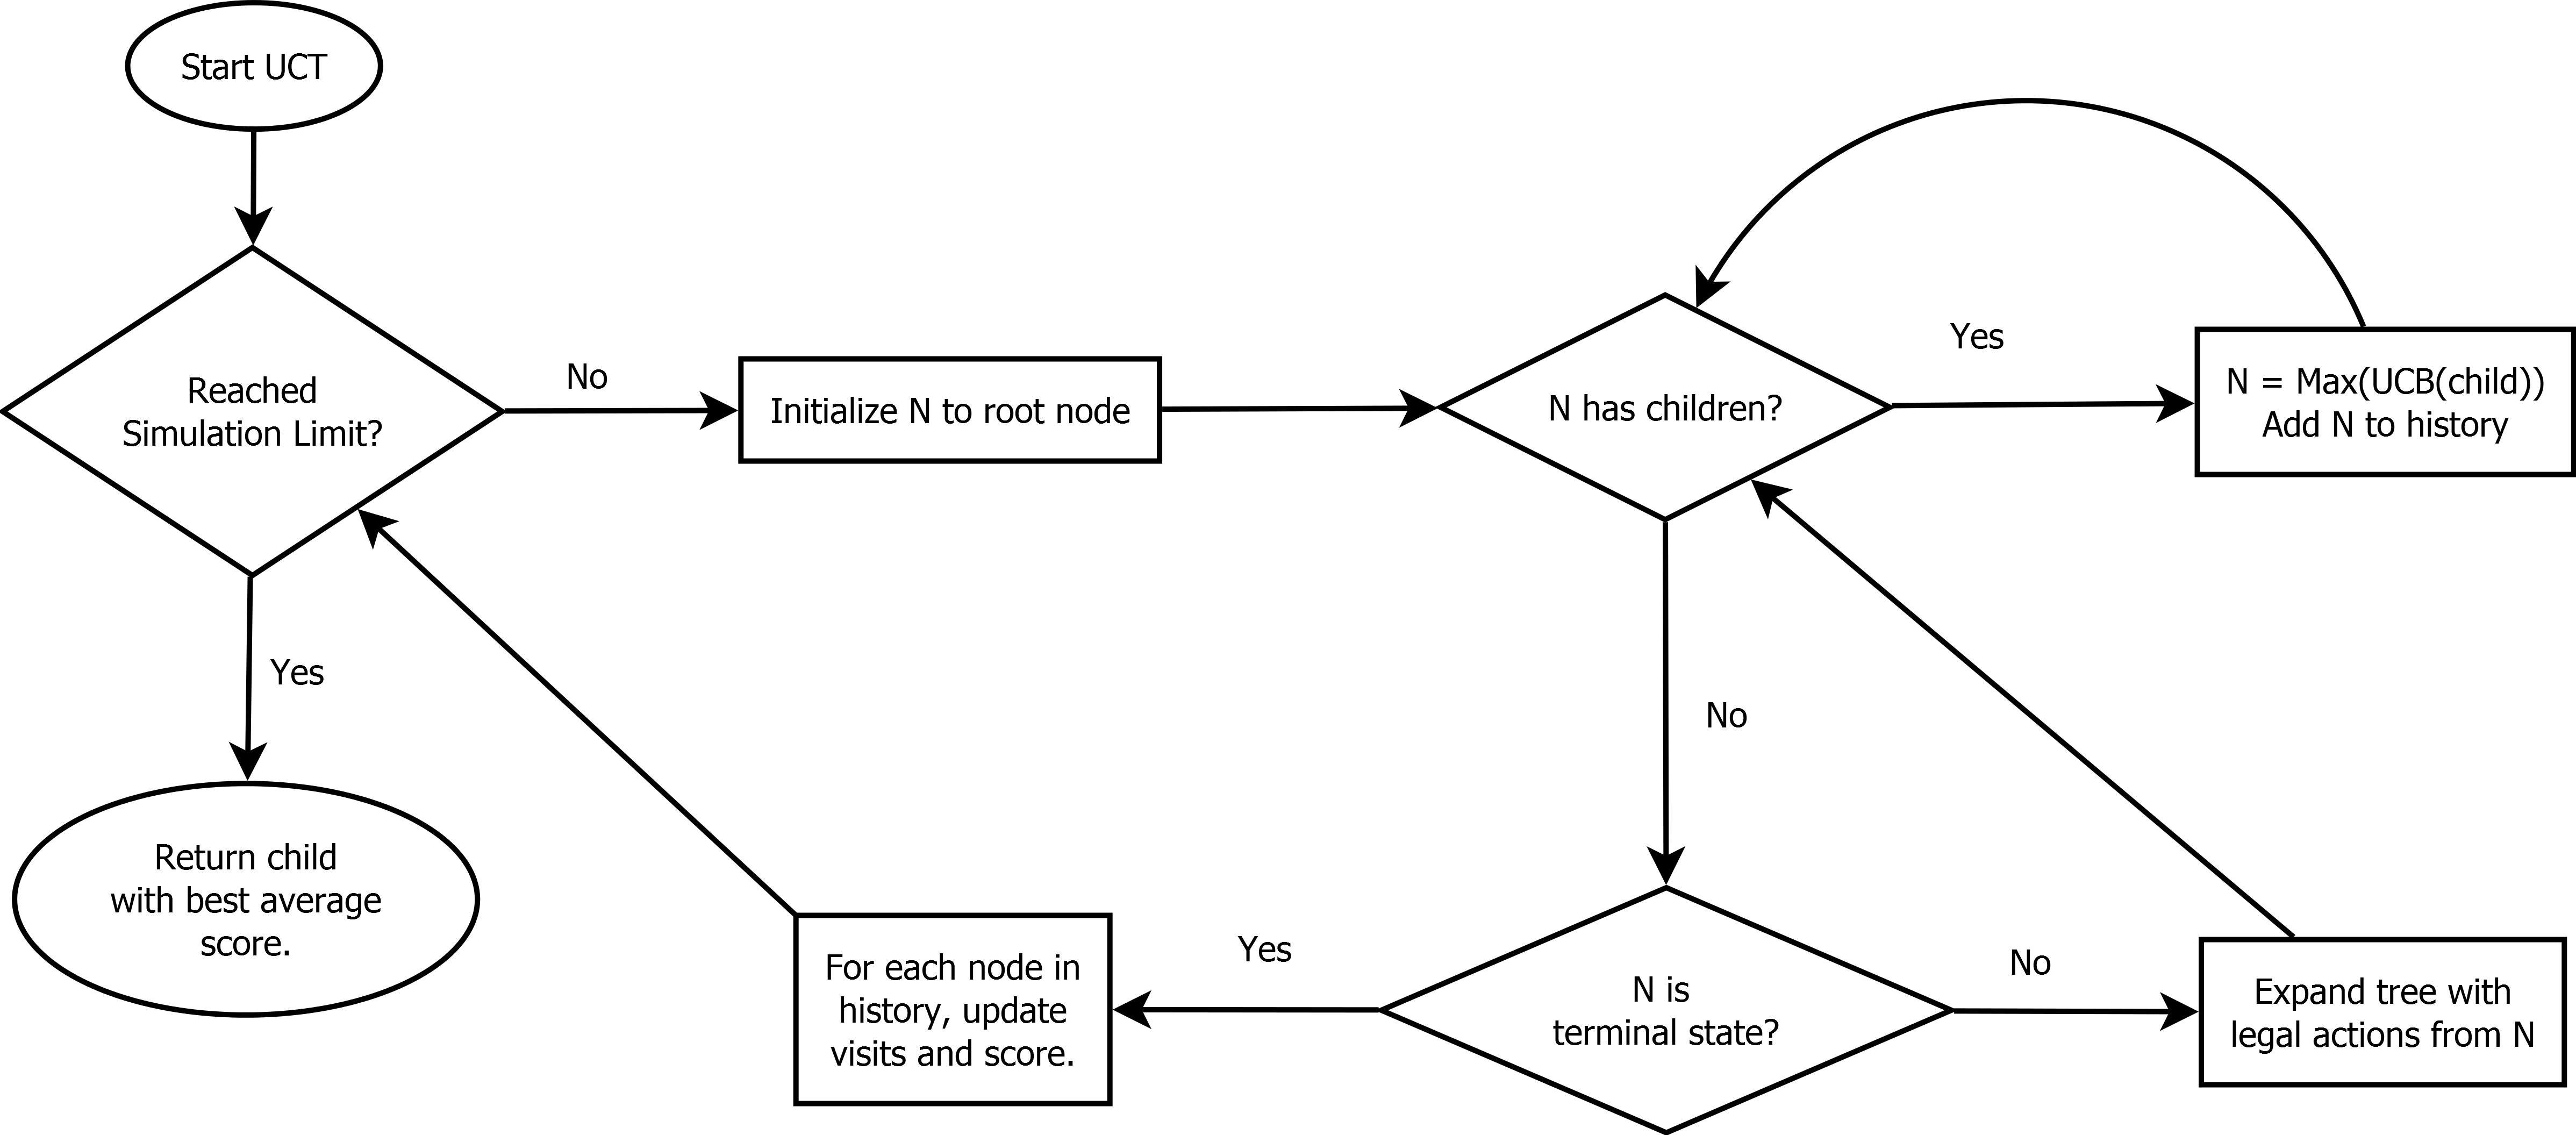
\includegraphics[width=\linewidth]{uct.png}
\caption{The basic UCT algorithm for searching over an MDP.  \ref{eqn:uct} is
the UCB algorithm referenced in the child selection step.}
\label{uct-diagram}
\end{figure}

A recently popular PP algorithm is the Upper Confidence bound applied to Trees (UCT)\cite{kocsis_bandit_2006}.
This algorithm is detailed in Figure \ref{uct-diagram}.
Online planning in MDPs generally follows two steps. From each state
encountered, a lookahead tree is constructed and used to estimate the
utility of each action in this state. Then, the best action is taken,
the system transitions to the next state and the procedure is
repeated. In order to build a lookahead tree, a ``rollout policy'' is
used. This policy has two components: if it encounters a state already
in the tree, it follows a ``tree policy,'' discussed further below. If
it encounters a new state, the policy reverts to a ``default'' policy
that typically randomly samples an action. In all cases, any rewards
received during the rollout search are backed up. Because this is a
Monte Carlo estimate, typically, several simultaneous trials are run,
and we keep track of the rewards received by each choice and
use this to select the best action at the root.

The final detail that UCT specifies is the method for determining the tree policy.
The tree policy needed by UCT for a state $s$ is the action $a$ in that state which maximizes:
\begin{equation}
P(s,a) = Q(s,a) + c\sqrt{\frac{ln N(s)}{N(s,a)}}\label{eqn:uct}
\end{equation}
Here $Q(s,a)$ is the estimated value of $a$ as observed in the tree
search and $N(s)$ and $N(s,a)$ are visit counts for the state and
state-action pair. Thus the second term is an exploration term that
biases the algorithm towards visiting actions that have not been
explored enough. $c$ is a constant that trades off exploration and
exploitation. This essentially treats each action decision
as a ``bandit problem" where the best action is determined by iteratively
exploring the branches of the action tree that previous experiments
have shown to be best.  Previous work \cite{uct-go} shows that this approach can
efficiently select near-optimal actions at each state.


\section{Natural Language Grammars}

A grammar is a set of rules which define strings that are contained within a language.
Many artificial languages, especially programming languages like C or Java, have
grammars which can be expressed concisely and without ambiguity.  Some
constructed languages, like Lojban \cite{lojban}, also have this property.

Natural languages (e.g. English), however, are well-known to have grammars which are difficult
to represent with any single given formalism \cite{klein2012context}. There are many possible
formalisms which can contain the rules that make up
a grammar.  Most of these formalisms involve a form of "rewriting", which
is to say, replacing a nonterminal token in a string with a specific set of
terminals and nonterminals.

\subsection{Context-Free Grammars}

One of the simplest grammars which can convey relationships between terminals
and nonterminals is the "Context Free Grammar" (CFG).  A CFG is made up of rules,
each of which specifies a possible rewrite of a nonterminal into one or more
terminals or nonterminals.  Once there are no further nonterminals to be rewritten,
the final state is a series of terminals which is in the language defined by the grammar.
This language is defined as the set of all possible generated sentences.

CFGs are so named because the rules in them are unable to consider the "context" for
their rewriting.  No rules may condition on the presence or placement of terminals
or nonterminals other than the single nonterminal to be rewritten.  This is, of course,
insufficiently expressive to be a grammar for English (or another natural language)\cite{jurafsky_textbook}.

One attempt to make CFGs more realistic for parsing or generating natural languages was to
introduce a probabilistic component.  This does not make CFGs any more expressive, but it
does help to cut down on the large number of potential parses for any given sentence
(English being a highly ambiguous language) by providing some direction as to which constructions
should be considered first.  In a Probabilistic Context Free Grammar (PCFG) \cite{pcfg_textbook}, CFG
rules are tagged with probabilities, usually representing the frequency of their appearance in
an observed corpus.  These probabilities are required to sum to 1 for each nonterminal to
be rewritten, so that there is a defined probability distribution over the options for each nonterminal.

This grammar type does appropriately convey the crucial truth that that not all rules are equal.
However, it does so in a  na\"{\i}ve way, unable to express these probabilities in terms of the placement
of the nonterminal in a sentence, and consequently also unable to successfully express English.

\subsection{Tree Adjoining Grammars}

A Tree Adjoining Grammar (TAG) takes a different approach, differing substantially from CFGs and PCFGs.
TAGs are tree-based grammars consisting of two sets of trees, called initial
trees and adjoining trees (sometimes ``auxiliary trees").  These two kinds of trees tend to perform
different roles semantically in addition to their differing syntactic roles.  The former,
initial trees, are usually for adding new semantic information to the sentence.  They
add new nodes to the sentence tree.  In a simplified TAG of English,
initial trees contain rules like ``Verb Phrases contain a Verb and a Noun", or ``VP $\rightarrow$ V N".
A sentence can be made entirely of initial trees, but a sentence must contain at least
one initial tree.  An example of an initial tree is shown in Figure \ref{initial-tree-example}.

\begin{figure}[ht]
\centering
\begin{minipage}[b]{0.45\linewidth}
\centering
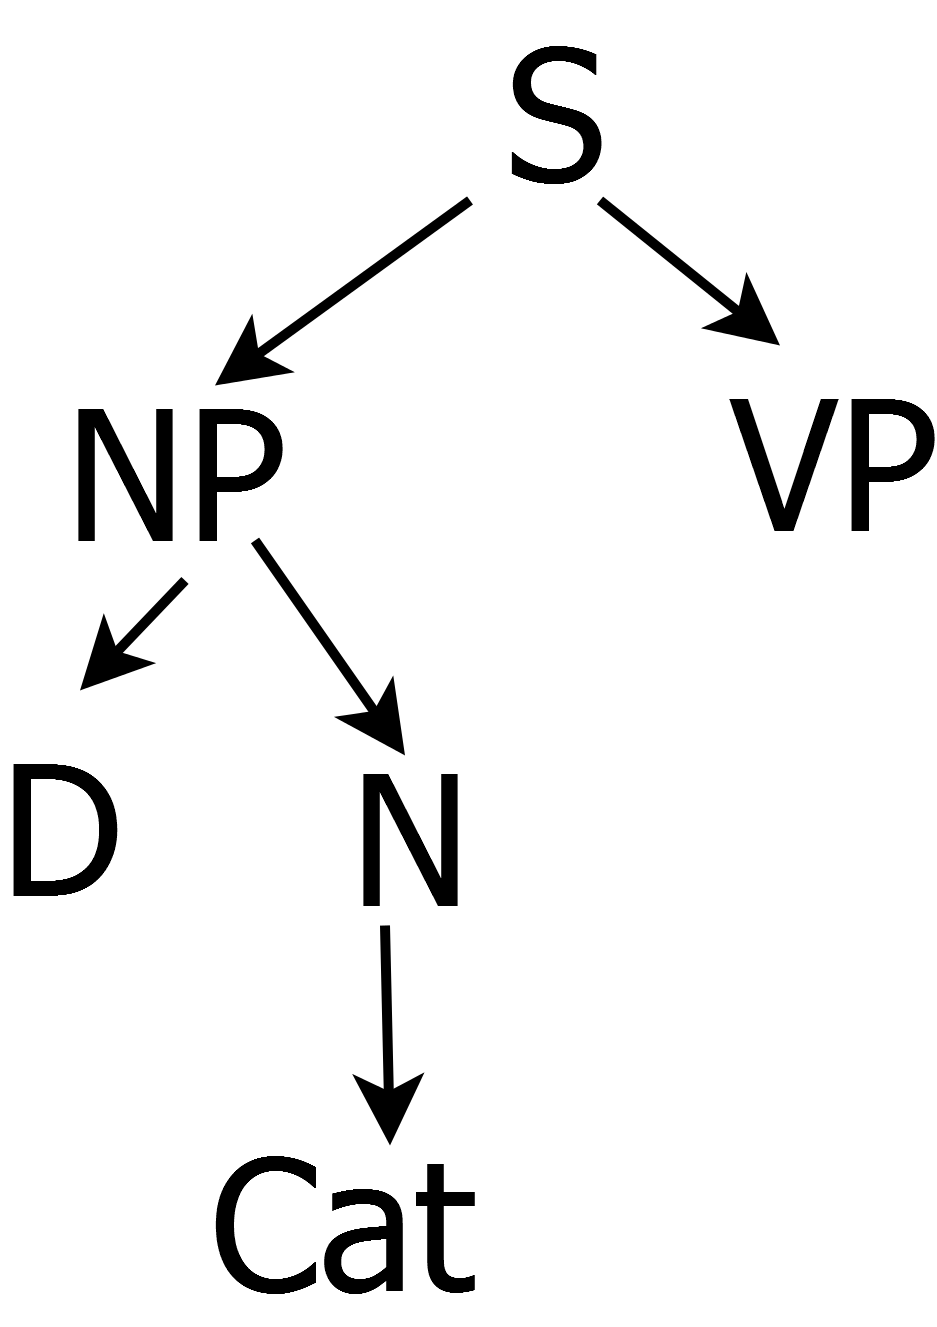
\includegraphics{initial-example.png}
\caption{An example of an initial tree in a lexicalized tree adjoining grammar}
\label{initial-tree-example}
\end{minipage}
\quad
\begin{minipage}[b]{0.45\linewidth}
\centering
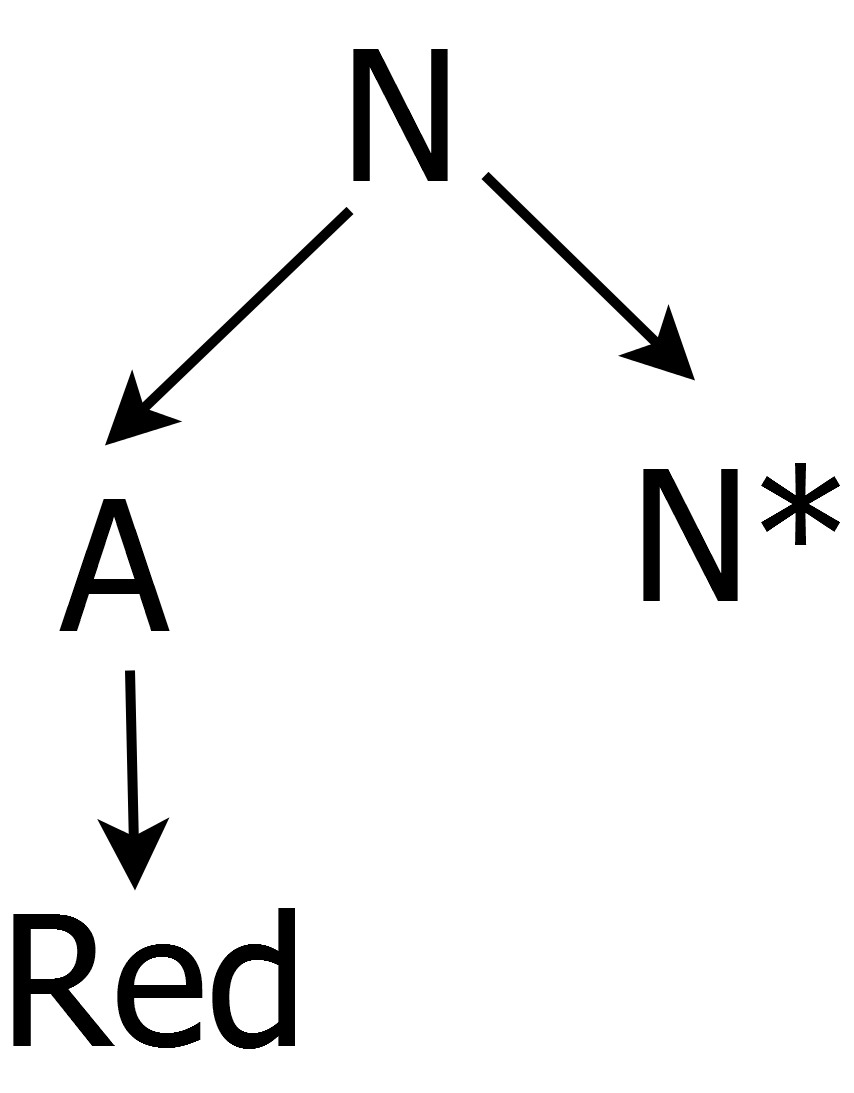
\includegraphics{adjoining-tree-example.png}
\caption{An example of an adjoining tree in a lexicalized tree adjoining grammar}
\label{adjoining-tree-example}
\end{minipage}
\end{figure}

This tree has as its root the S node, and this defines how it can interact with other
trees under a TAG.  Since this is an initial tree, it can only interact with other trees by
substitution.  That is, this tree is a drop-in replacement for an S node with no children.
This is how we get from our stub sentence (S) to a complete sentence.

Adjoining trees usually clarify a point in a sentence.  In a simplified TAG of English, adjoining
trees would contain rules like ``a noun can have an adjective placed in front of it," or ``N $\rightarrow$ A N".
An example of an adjoining tree is shown in Figure \ref{adjoining-tree-example}.

This tree has as its root an N node.  It also has a specially annotated N node elsewhere in the
tree.  These nodes define its interaction with other trees under a TAG.  Adjoining trees interact
with other trees only by "adjoining".  In an adjoining action, we select the node
to adjoin to, which must be of the same label as the root node of the adjoining tree.  We remove
that node from the other tree and put the adjoining tree in its place.  Then
we place that original node into the adjoining tree as a substitution for the foot node.
For example, if we had the tree in Figure \ref{tree-1} and we wanted to adjoin the example adjoining tree
in Figure \ref{adjoining-tree-example}, we would first create the intermediate tree in Figure \ref{tree-2},
and then perform the substitution and get the tree in Figure \ref{tree-3}.  Notice that this has the effect,
in all cases, of making the tree deeper.

\begin{figure}[ht]
\centering
\begin{minipage}[b]{0.3\linewidth}
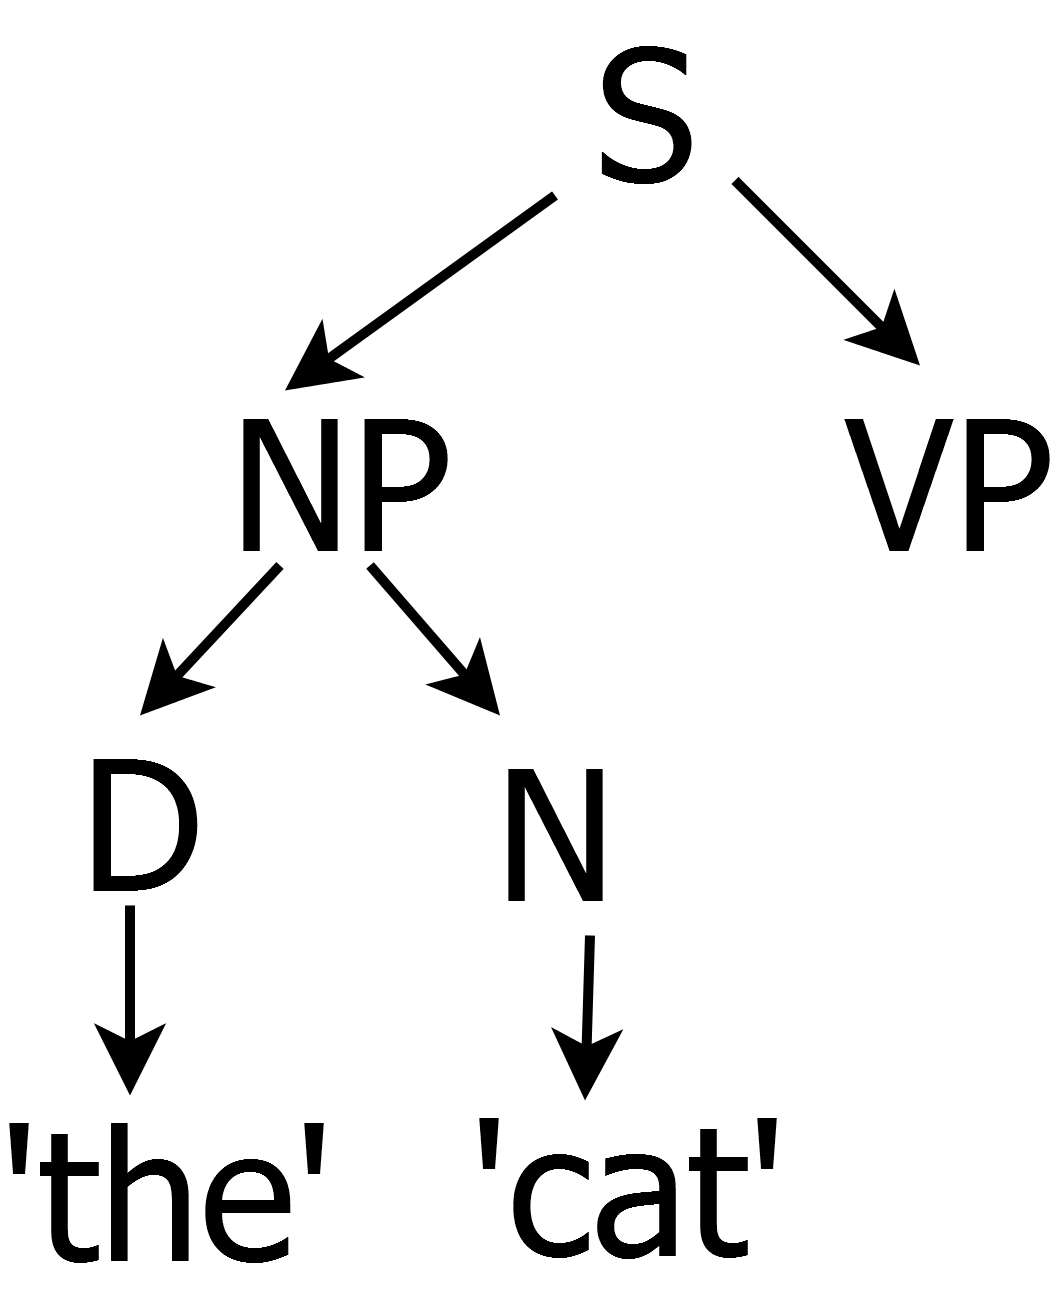
\includegraphics{tree-1.png}
\caption{Partial tree}
\label{tree-1}
\end{minipage}
\quad
\begin{minipage}[b]{0.3\linewidth}
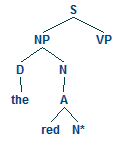
\includegraphics{tree-2.png}
\caption{Intermediate tree}
\label{tree-2}
\end{minipage}
\quad
\begin{minipage}[b]{0.3\linewidth}
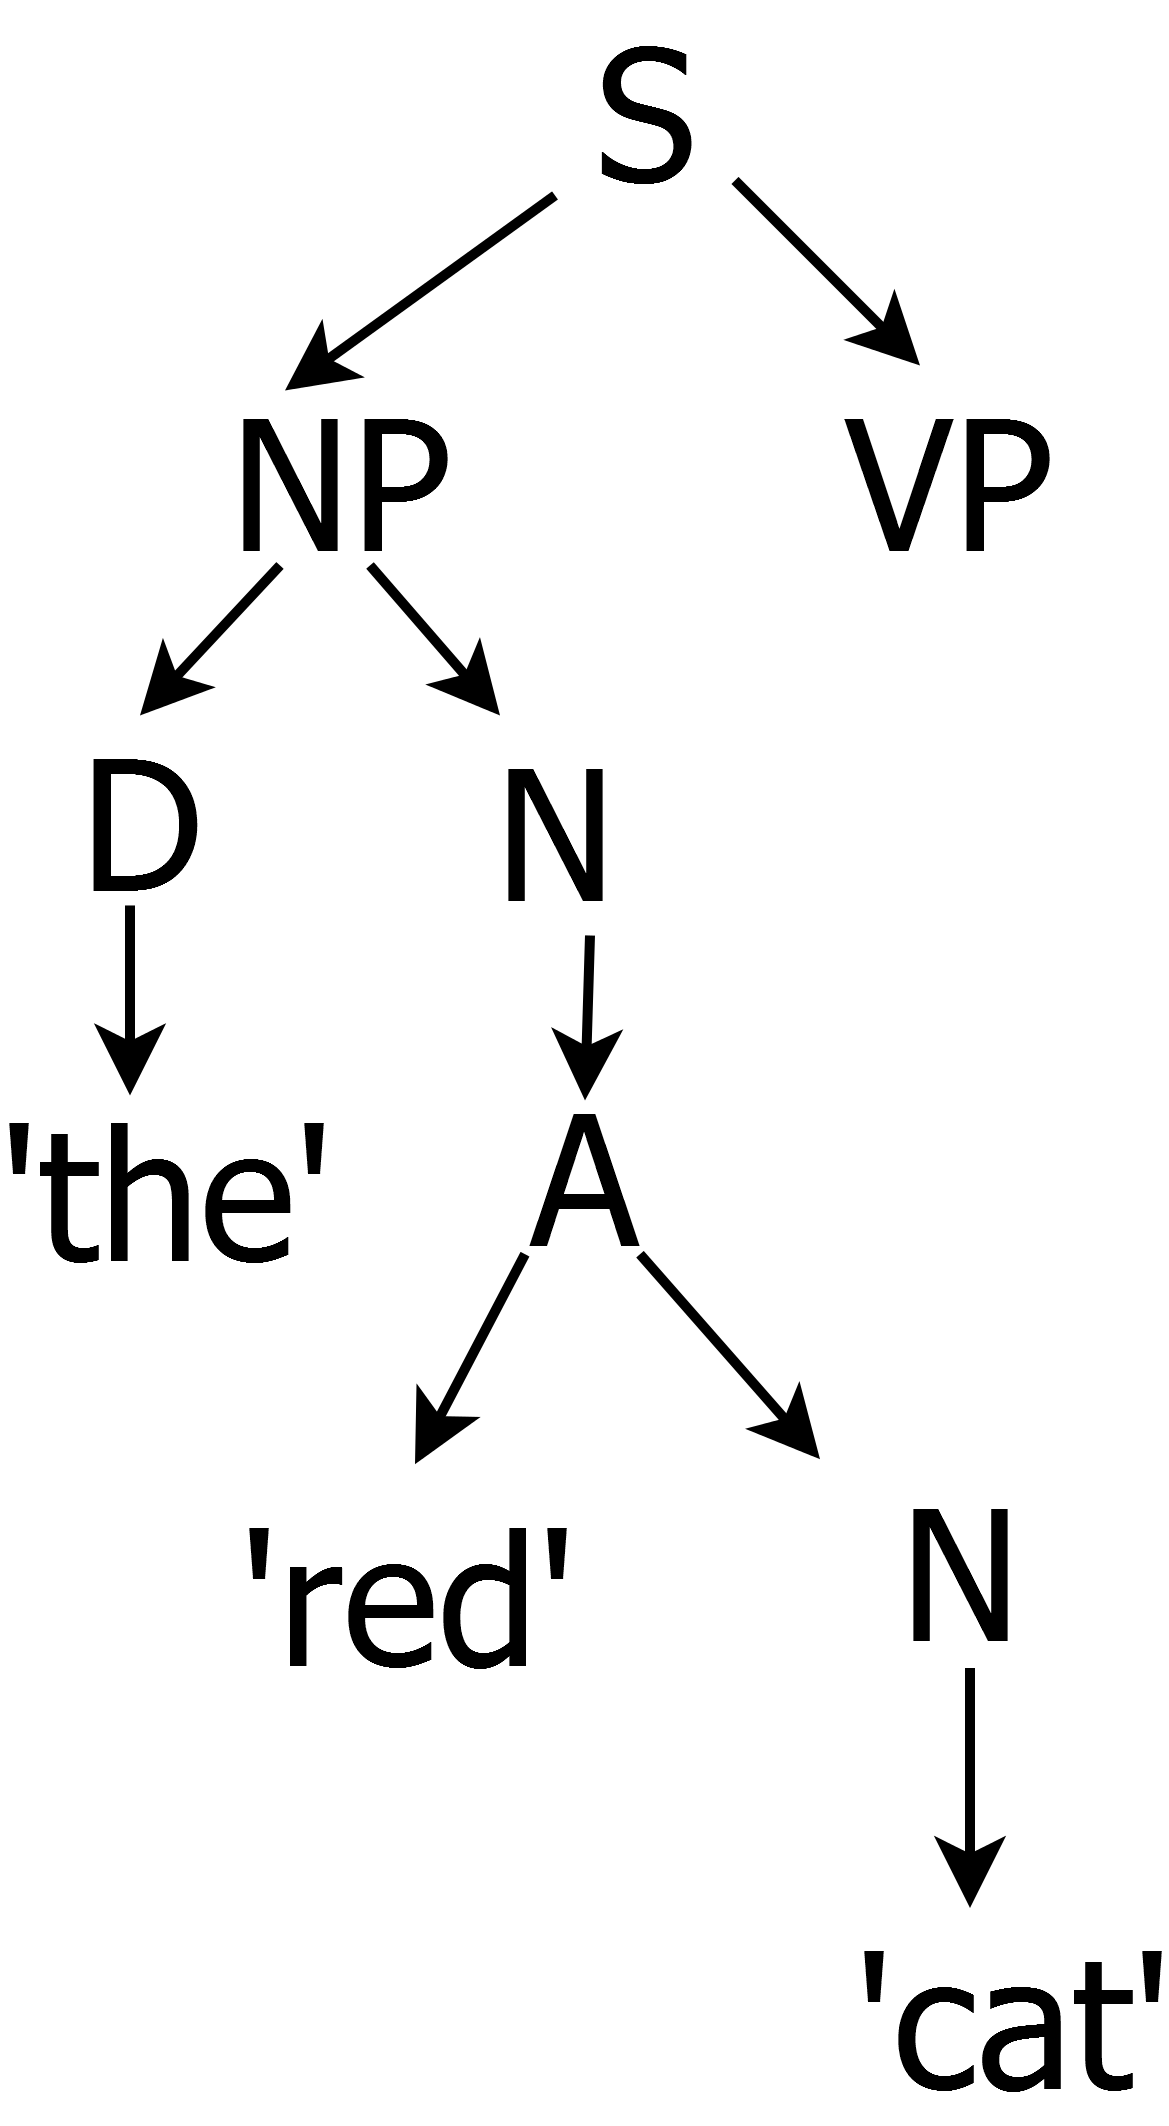
\includegraphics{tree-3.png}
\caption{Final tree}
\label{tree-3}
\end{minipage}
\end{figure}

We use a variation of TAGs in our work, called a lexicalized TAG (LTAG), where each tree is
associated with a lexical item called an anchor.  All examples given above are examples of
lexicalized trees.  An example of an unlexicalized tree would be (NP (D) (N)), where there
are no nodes containing lexical tokens.

As with CFGs, an attempt to make TAGs easier to use for generation or parsing was to
introduce probabilities.  Each tree rule in a TAG must be annotated with a probability, and
there will be a probability distribution for each nonterminal at the frontier of the tree.
These probabilistic TAGs, or PTAGs, can be useful if a corpus of text is available.

The XTAG project has had some success using LTAGs to model English grammar\cite{xtag}, 
so we focus mostly on LTAGs in our work.